\subsection{Methodology} \label{Methodology}

The probabilistic graph is converted into a deterministic instance through sampling. Each uncertain parameter, like obstacle positioning, is constructing by drawing from its probability distribution. Uncertainty gets reduced into a single concrete scenario, enabling deterministic emulation and evaluation. Multiple such samples are generated to well-approximate the probability distribution, and accordingly well-quantify our decision making mechanism on the decided path outcomes. Metrics include collisions, lives lost, traffic laws violations. Statistical measures include expected total harm or reward, and variance.

\tikzset{every picture/.style={line width=0.75pt}} %set default line width to 0.75pt        

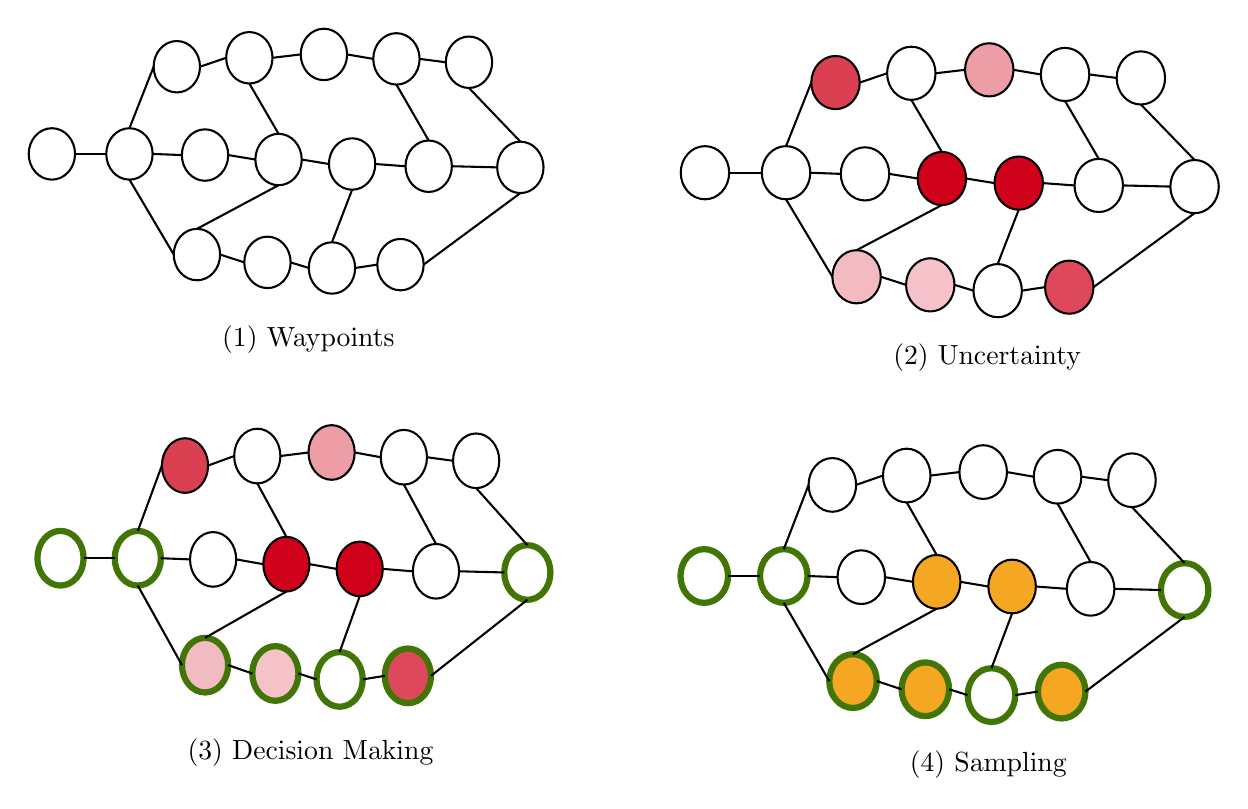
\begin{tikzpicture}[x=0.75pt,y=0.75pt,yscale=-1,xscale=1]
%uncomment if require: \path (0,405); %set diagram left start at 0, and has height of 405

%Shape: Ellipse [id:dp6172494245642979] 
\draw   (10.96,70.33) .. controls (10.96,63.49) and (15.95,57.94) .. (22.12,57.94) .. controls (28.29,57.94) and (33.28,63.49) .. (33.28,70.33) .. controls (33.28,77.17) and (28.29,82.72) .. (22.12,82.72) .. controls (15.95,82.72) and (10.96,77.17) .. (10.96,70.33) -- cycle ;
%Shape: Ellipse [id:dp1152670128331501] 
\draw   (48.33,70.33) .. controls (48.33,63.49) and (53.33,57.94) .. (59.5,57.94) .. controls (65.66,57.94) and (70.66,63.49) .. (70.66,70.33) .. controls (70.66,77.17) and (65.66,82.72) .. (59.5,82.72) .. controls (53.33,82.72) and (48.33,77.17) .. (48.33,70.33) -- cycle ;
%Shape: Ellipse [id:dp5590595997056589] 
\draw   (84.74,70.87) .. controls (84.74,64.03) and (89.74,58.48) .. (95.9,58.48) .. controls (102.07,58.48) and (107.07,64.03) .. (107.07,70.87) .. controls (107.07,77.71) and (102.07,83.26) .. (95.9,83.26) .. controls (89.74,83.26) and (84.74,77.71) .. (84.74,70.87) -- cycle ;
%Shape: Ellipse [id:dp5011939728441563] 
\draw   (120.17,73.03) .. controls (120.17,66.18) and (125.17,60.64) .. (131.34,60.64) .. controls (137.5,60.64) and (142.5,66.18) .. (142.5,73.03) .. controls (142.5,79.87) and (137.5,85.41) .. (131.34,85.41) .. controls (125.17,85.41) and (120.17,79.87) .. (120.17,73.03) -- cycle ;
%Shape: Ellipse [id:dp7413016599095847] 
\draw   (80.85,118.81) .. controls (80.85,111.97) and (85.85,106.42) .. (92.02,106.42) .. controls (98.19,106.42) and (103.18,111.97) .. (103.18,118.81) .. controls (103.18,125.66) and (98.19,131.2) .. (92.02,131.2) .. controls (85.85,131.2) and (80.85,125.66) .. (80.85,118.81) -- cycle ;
%Shape: Ellipse [id:dp26941055046572315] 
\draw   (114.83,122.58) .. controls (114.83,115.74) and (119.83,110.19) .. (126,110.19) .. controls (132.16,110.19) and (137.16,115.74) .. (137.16,122.58) .. controls (137.16,129.43) and (132.16,134.97) .. (126,134.97) .. controls (119.83,134.97) and (114.83,129.43) .. (114.83,122.58) -- cycle ;
%Shape: Ellipse [id:dp13128192047796583] 
\draw   (145.9,125.28) .. controls (145.9,118.43) and (150.9,112.89) .. (157.06,112.89) .. controls (163.23,112.89) and (168.23,118.43) .. (168.23,125.28) .. controls (168.23,132.12) and (163.23,137.67) .. (157.06,137.67) .. controls (150.9,137.67) and (145.9,132.12) .. (145.9,125.28) -- cycle ;
%Shape: Ellipse [id:dp12509773375527322] 
\draw   (106.1,24.01) .. controls (106.1,17.16) and (111.09,11.62) .. (117.26,11.62) .. controls (123.43,11.62) and (128.42,17.16) .. (128.42,24.01) .. controls (128.42,30.85) and (123.43,36.4) .. (117.26,36.4) .. controls (111.09,36.4) and (106.1,30.85) .. (106.1,24.01) -- cycle ;
%Shape: Ellipse [id:dp591811656416317] 
\draw   (178.91,123.66) .. controls (178.91,116.82) and (183.91,111.27) .. (190.07,111.27) .. controls (196.24,111.27) and (201.24,116.82) .. (201.24,123.66) .. controls (201.24,130.5) and (196.24,136.05) .. (190.07,136.05) .. controls (183.91,136.05) and (178.91,130.5) .. (178.91,123.66) -- cycle ;
%Shape: Ellipse [id:dp7250601409314574] 
\draw   (71.15,28.32) .. controls (71.15,21.47) and (76.14,15.93) .. (82.31,15.93) .. controls (88.48,15.93) and (93.48,21.47) .. (93.48,28.32) .. controls (93.48,35.16) and (88.48,40.7) .. (82.31,40.7) .. controls (76.14,40.7) and (71.15,35.16) .. (71.15,28.32) -- cycle ;
%Shape: Ellipse [id:dp4062584198990371] 
\draw   (155.61,75.18) .. controls (155.61,68.34) and (160.61,62.79) .. (166.77,62.79) .. controls (172.94,62.79) and (177.94,68.34) .. (177.94,75.18) .. controls (177.94,82.02) and (172.94,87.57) .. (166.77,87.57) .. controls (160.61,87.57) and (155.61,82.02) .. (155.61,75.18) -- cycle ;
%Shape: Ellipse [id:dp5782111529794598] 
\draw   (192.5,76.26) .. controls (192.5,69.41) and (197.5,63.87) .. (203.66,63.87) .. controls (209.83,63.87) and (214.83,69.41) .. (214.83,76.26) .. controls (214.83,83.1) and (209.83,88.65) .. (203.66,88.65) .. controls (197.5,88.65) and (192.5,83.1) .. (192.5,76.26) -- cycle ;
%Shape: Ellipse [id:dp695651539314398] 
\draw   (142.02,22.39) .. controls (142.02,15.55) and (147.01,10) .. (153.18,10) .. controls (159.35,10) and (164.35,15.55) .. (164.35,22.39) .. controls (164.35,29.23) and (159.35,34.78) .. (153.18,34.78) .. controls (147.01,34.78) and (142.02,29.23) .. (142.02,22.39) -- cycle ;
%Shape: Ellipse [id:dp8789609630879338] 
\draw   (176.97,24.54) .. controls (176.97,17.7) and (181.96,12.15) .. (188.13,12.15) .. controls (194.3,12.15) and (199.29,17.7) .. (199.29,24.54) .. controls (199.29,31.39) and (194.3,36.93) .. (188.13,36.93) .. controls (181.96,36.93) and (176.97,31.39) .. (176.97,24.54) -- cycle ;
%Shape: Ellipse [id:dp39873863665216325] 
\draw   (211.92,26.16) .. controls (211.92,19.32) and (216.91,13.77) .. (223.08,13.77) .. controls (229.25,13.77) and (234.24,19.32) .. (234.24,26.16) .. controls (234.24,33) and (229.25,38.55) .. (223.08,38.55) .. controls (216.91,38.55) and (211.92,33) .. (211.92,26.16) -- cycle ;
%Straight Lines [id:da6795031886711704] 
\draw    (33.28,70.33) -- (48.33,70.33) ;
%Straight Lines [id:da24870539515316903] 
\draw    (70.66,70.33) -- (84.74,70.87) ;
%Straight Lines [id:da8519484585152293] 
\draw    (107.07,70.87) -- (120.17,73.03) ;
%Straight Lines [id:da7097521095055688] 
\draw    (142.5,73.03) -- (155.61,75.18) ;
%Straight Lines [id:da632635038672595] 
\draw    (177.94,75.18) -- (192.5,76.26) ;
%Straight Lines [id:da3411812205003839] 
\draw    (59.5,57.94) -- (71.15,28.32) ;
%Straight Lines [id:da5259680917016067] 
\draw    (93.48,28.32) -- (106.1,24.01) ;
%Straight Lines [id:da5637620273305417] 
\draw    (128.42,24.01) -- (142.02,22.39) ;
%Straight Lines [id:da15489769967685163] 
\draw    (117.26,36.4) -- (131.34,60.64) ;
%Straight Lines [id:da6681848193571542] 
\draw    (164.35,22.39) -- (176.97,24.54) ;
%Straight Lines [id:da3556048835390373] 
\draw    (199.29,24.54) -- (211.92,26.16) ;
%Straight Lines [id:da44413658850259674] 
\draw    (59.5,82.72) -- (80.85,118.81) ;
%Straight Lines [id:da48625901624637] 
\draw    (103.18,118.81) -- (114.83,122.58) ;
%Straight Lines [id:da8028559161112461] 
\draw    (137.16,122.58) -- (145.9,125.28) ;
%Straight Lines [id:da4239150618132703] 
\draw    (168.23,125.28) -- (178.91,123.66) ;
%Straight Lines [id:da9182804115752854] 
\draw    (188.13,36.93) -- (203.66,63.87) ;
%Straight Lines [id:da5847694764870806] 
\draw    (157.06,112.89) -- (166.77,87.57) ;
%Straight Lines [id:da9255723298513319] 
\draw    (92.02,106.42) -- (131.34,85.41) ;
%Shape: Ellipse [id:dp37476525267271144] 
\draw   (236.67,76.8) .. controls (236.67,69.95) and (241.67,64.41) .. (247.84,64.41) .. controls (254,64.41) and (259,69.95) .. (259,76.8) .. controls (259,83.64) and (254,89.19) .. (247.84,89.19) .. controls (241.67,89.19) and (236.67,83.64) .. (236.67,76.8) -- cycle ;
%Straight Lines [id:da10095243498955253] 
\draw    (201.24,123.66) -- (247.84,89.19) ;
%Straight Lines [id:da7732871806968082] 
\draw    (214.83,76.26) -- (236.67,76.8) ;
%Straight Lines [id:da22351855506704865] 
\draw    (223.08,38.55) -- (247.84,64.41) ;
%Shape: Ellipse [id:dp16583991508781892] 
\draw   (325.11,79.38) .. controls (325.11,72.3) and (330.33,66.57) .. (336.77,66.57) .. controls (343.22,66.57) and (348.44,72.3) .. (348.44,79.38) .. controls (348.44,86.45) and (343.22,92.19) .. (336.77,92.19) .. controls (330.33,92.19) and (325.11,86.45) .. (325.11,79.38) -- cycle ;
%Shape: Ellipse [id:dp6966948952933287] 
\draw   (364.17,79.38) .. controls (364.17,72.3) and (369.39,66.57) .. (375.84,66.57) .. controls (382.28,66.57) and (387.5,72.3) .. (387.5,79.38) .. controls (387.5,86.45) and (382.28,92.19) .. (375.84,92.19) .. controls (369.39,92.19) and (364.17,86.45) .. (364.17,79.38) -- cycle ;
%Shape: Ellipse [id:dp4272766063501725] 
\draw   (402.21,79.94) .. controls (402.21,72.86) and (407.44,67.13) .. (413.88,67.13) .. controls (420.33,67.13) and (425.55,72.86) .. (425.55,79.94) .. controls (425.55,87.01) and (420.33,92.75) .. (413.88,92.75) .. controls (407.44,92.75) and (402.21,87.01) .. (402.21,79.94) -- cycle ;
%Shape: Ellipse [id:dp029675346165769945] 
\draw  [fill={rgb, 255:red, 208; green, 2; blue, 27 }  ,fill opacity=1 ] (439.25,82.16) .. controls (439.25,75.09) and (444.47,69.35) .. (450.91,69.35) .. controls (457.36,69.35) and (462.58,75.09) .. (462.58,82.16) .. controls (462.58,89.24) and (457.36,94.97) .. (450.91,94.97) .. controls (444.47,94.97) and (439.25,89.24) .. (439.25,82.16) -- cycle ;
%Shape: Ellipse [id:dp9798739627585888] 
\draw  [fill={rgb, 255:red, 208; green, 2; blue, 27 }  ,fill opacity=0.27 ] (398.16,129.51) .. controls (398.16,122.43) and (403.38,116.7) .. (409.82,116.7) .. controls (416.27,116.7) and (421.49,122.43) .. (421.49,129.51) .. controls (421.49,136.58) and (416.27,142.32) .. (409.82,142.32) .. controls (403.38,142.32) and (398.16,136.58) .. (398.16,129.51) -- cycle ;
%Shape: Ellipse [id:dp9652797031979226] 
\draw  [fill={rgb, 255:red, 208; green, 2; blue, 27 }  ,fill opacity=0.24 ] (433.67,133.41) .. controls (433.67,126.33) and (438.89,120.59) .. (445.33,120.59) .. controls (451.78,120.59) and (457,126.33) .. (457,133.41) .. controls (457,140.48) and (451.78,146.22) .. (445.33,146.22) .. controls (438.89,146.22) and (433.67,140.48) .. (433.67,133.41) -- cycle ;
%Shape: Ellipse [id:dp6613978913898011] 
\draw   (466.13,136.19) .. controls (466.13,129.12) and (471.36,123.38) .. (477.8,123.38) .. controls (484.25,123.38) and (489.47,129.12) .. (489.47,136.19) .. controls (489.47,143.26) and (484.25,149) .. (477.8,149) .. controls (471.36,149) and (466.13,143.26) .. (466.13,136.19) -- cycle ;
%Shape: Ellipse [id:dp9691042482642522] 
\draw   (424.54,31.48) .. controls (424.54,24.41) and (429.76,18.67) .. (436.2,18.67) .. controls (442.65,18.67) and (447.87,24.41) .. (447.87,31.48) .. controls (447.87,38.56) and (442.65,44.29) .. (436.2,44.29) .. controls (429.76,44.29) and (424.54,38.56) .. (424.54,31.48) -- cycle ;
%Shape: Ellipse [id:dp6300141737135296] 
\draw  [fill={rgb, 255:red, 208; green, 2; blue, 27 }  ,fill opacity=0.72 ] (500.63,134.52) .. controls (500.63,127.44) and (505.85,121.71) .. (512.3,121.71) .. controls (518.74,121.71) and (523.97,127.44) .. (523.97,134.52) .. controls (523.97,141.59) and (518.74,147.33) .. (512.3,147.33) .. controls (505.85,147.33) and (500.63,141.59) .. (500.63,134.52) -- cycle ;
%Shape: Ellipse [id:dp6526656142861484] 
\draw  [fill={rgb, 255:red, 208; green, 2; blue, 27 }  ,fill opacity=0.76 ] (388.01,35.94) .. controls (388.01,28.86) and (393.23,23.13) .. (399.68,23.13) .. controls (406.12,23.13) and (411.35,28.86) .. (411.35,35.94) .. controls (411.35,43.01) and (406.12,48.75) .. (399.68,48.75) .. controls (393.23,48.75) and (388.01,43.01) .. (388.01,35.94) -- cycle ;
%Shape: Ellipse [id:dp8227295674221913] 
\draw  [fill={rgb, 255:red, 208; green, 2; blue, 27 }  ,fill opacity=1 ] (476.28,84.39) .. controls (476.28,77.32) and (481.5,71.58) .. (487.95,71.58) .. controls (494.39,71.58) and (499.62,77.32) .. (499.62,84.39) .. controls (499.62,91.47) and (494.39,97.2) .. (487.95,97.2) .. controls (481.5,97.2) and (476.28,91.47) .. (476.28,84.39) -- cycle ;
%Shape: Ellipse [id:dp42890645204098066] 
\draw   (514.83,85.51) .. controls (514.83,78.43) and (520.06,72.7) .. (526.5,72.7) .. controls (532.95,72.7) and (538.17,78.43) .. (538.17,85.51) .. controls (538.17,92.58) and (532.95,98.32) .. (526.5,98.32) .. controls (520.06,98.32) and (514.83,92.58) .. (514.83,85.51) -- cycle ;
%Shape: Ellipse [id:dp8571173419457159] 
\draw  [color={rgb, 255:red, 0; green, 0; blue, 0 }  ,draw opacity=1 ][fill={rgb, 255:red, 208; green, 2; blue, 27 }  ,fill opacity=0.39 ] (462.08,29.81) .. controls (462.08,22.74) and (467.3,17) .. (473.74,17) .. controls (480.19,17) and (485.41,22.74) .. (485.41,29.81) .. controls (485.41,36.88) and (480.19,42.62) .. (473.74,42.62) .. controls (467.3,42.62) and (462.08,36.88) .. (462.08,29.81) -- cycle ;
%Shape: Ellipse [id:dp1396922568717307] 
\draw   (498.6,32.04) .. controls (498.6,24.96) and (503.82,19.23) .. (510.27,19.23) .. controls (516.71,19.23) and (521.94,24.96) .. (521.94,32.04) .. controls (521.94,39.11) and (516.71,44.85) .. (510.27,44.85) .. controls (503.82,44.85) and (498.6,39.11) .. (498.6,32.04) -- cycle ;
%Shape: Ellipse [id:dp362329559602649] 
\draw   (535.13,33.71) .. controls (535.13,26.63) and (540.35,20.9) .. (546.79,20.9) .. controls (553.24,20.9) and (558.46,26.63) .. (558.46,33.71) .. controls (558.46,40.78) and (553.24,46.52) .. (546.79,46.52) .. controls (540.35,46.52) and (535.13,40.78) .. (535.13,33.71) -- cycle ;
%Straight Lines [id:da9585583850831978] 
\draw    (348.44,79.38) -- (364.17,79.38) ;
%Straight Lines [id:da008493881417554139] 
\draw    (387.5,79.38) -- (402.21,79.94) ;
%Straight Lines [id:da15361080323737553] 
\draw    (425.55,79.94) -- (439.25,82.16) ;
%Straight Lines [id:da9233926279062612] 
\draw    (462.58,82.16) -- (476.28,84.39) ;
%Straight Lines [id:da6882111407440119] 
\draw    (499.62,84.39) -- (514.83,85.51) ;
%Straight Lines [id:da7472421988031972] 
\draw    (375.84,66.57) -- (388.01,35.94) ;
%Straight Lines [id:da13991715605563781] 
\draw    (411.35,35.94) -- (424.54,31.48) ;
%Straight Lines [id:da7539380032549543] 
\draw    (447.87,31.48) -- (462.08,29.81) ;
%Straight Lines [id:da761448994391088] 
\draw    (436.2,44.29) -- (450.91,69.35) ;
%Straight Lines [id:da30644873418927165] 
\draw    (485.41,29.81) -- (498.6,32.04) ;
%Straight Lines [id:da7903543900265124] 
\draw    (521.94,32.04) -- (535.13,33.71) ;
%Straight Lines [id:da40008760043914315] 
\draw    (375.84,92.19) -- (398.16,129.51) ;
%Straight Lines [id:da3828066353585615] 
\draw    (421.49,129.51) -- (433.67,133.41) ;
%Straight Lines [id:da20290663297426326] 
\draw    (457,133.41) -- (466.13,136.19) ;
%Straight Lines [id:da7840234761748077] 
\draw    (489.47,136.19) -- (500.63,134.52) ;
%Straight Lines [id:da8820538644400171] 
\draw    (510.27,44.85) -- (526.5,72.7) ;
%Straight Lines [id:da28723470911001847] 
\draw    (477.8,123.38) -- (487.95,97.2) ;
%Straight Lines [id:da7825729102198125] 
\draw    (409.82,116.7) -- (450.91,94.97) ;
%Shape: Ellipse [id:dp95896654791443] 
\draw   (561,86.06) .. controls (561,78.99) and (566.22,73.25) .. (572.67,73.25) .. controls (579.11,73.25) and (584.33,78.99) .. (584.33,86.06) .. controls (584.33,93.14) and (579.11,98.87) .. (572.67,98.87) .. controls (566.22,98.87) and (561,93.14) .. (561,86.06) -- cycle ;
%Straight Lines [id:da1710745202798496] 
\draw    (523.97,134.52) -- (572.67,98.87) ;
%Straight Lines [id:da40515562568446395] 
\draw    (538.17,85.51) -- (561,86.06) ;
%Straight Lines [id:da35151625683479404] 
\draw    (546.79,46.52) -- (572.67,73.25) ;
%Shape: Ellipse [id:dp9407843988416862] 
\draw  [color={rgb, 255:red, 65; green, 117; blue, 5 }  ,draw opacity=1 ][line width=2.25]  (15.15,265.11) .. controls (15.15,257.84) and (20.13,251.95) .. (26.27,251.95) .. controls (32.42,251.95) and (37.4,257.84) .. (37.4,265.11) .. controls (37.4,272.38) and (32.42,278.28) .. (26.27,278.28) .. controls (20.13,278.28) and (15.15,272.38) .. (15.15,265.11) -- cycle ;
%Shape: Ellipse [id:dp14535557248848296] 
\draw  [color={rgb, 255:red, 65; green, 117; blue, 5 }  ,draw opacity=1 ][line width=2.25]  (52.4,265.11) .. controls (52.4,257.84) and (57.38,251.95) .. (63.52,251.95) .. controls (69.67,251.95) and (74.65,257.84) .. (74.65,265.11) .. controls (74.65,272.38) and (69.67,278.28) .. (63.52,278.28) .. controls (57.38,278.28) and (52.4,272.38) .. (52.4,265.11) -- cycle ;
%Shape: Ellipse [id:dp6265950750273022] 
\draw   (88.68,265.68) .. controls (88.68,258.41) and (93.66,252.52) .. (99.8,252.52) .. controls (105.95,252.52) and (110.93,258.41) .. (110.93,265.68) .. controls (110.93,272.96) and (105.95,278.85) .. (99.8,278.85) .. controls (93.66,278.85) and (88.68,272.96) .. (88.68,265.68) -- cycle ;
%Shape: Ellipse [id:dp007425727658135539] 
\draw  [fill={rgb, 255:red, 208; green, 2; blue, 27 }  ,fill opacity=1 ] (123.99,267.97) .. controls (123.99,260.7) and (128.97,254.81) .. (135.11,254.81) .. controls (141.26,254.81) and (146.24,260.7) .. (146.24,267.97) .. controls (146.24,275.25) and (141.26,281.14) .. (135.11,281.14) .. controls (128.97,281.14) and (123.99,275.25) .. (123.99,267.97) -- cycle ;
%Shape: Ellipse [id:dp8285304855470328] 
\draw  [color={rgb, 255:red, 65; green, 117; blue, 5 }  ,draw opacity=1 ][fill={rgb, 255:red, 208; green, 2; blue, 27 }  ,fill opacity=0.27 ][line width=2.25]  (84.81,316.63) .. controls (84.81,309.36) and (89.79,303.47) .. (95.93,303.47) .. controls (102.08,303.47) and (107.06,309.36) .. (107.06,316.63) .. controls (107.06,323.9) and (102.08,329.8) .. (95.93,329.8) .. controls (89.79,329.8) and (84.81,323.9) .. (84.81,316.63) -- cycle ;
%Shape: Ellipse [id:dp9976808030994382] 
\draw  [color={rgb, 255:red, 65; green, 117; blue, 5 }  ,draw opacity=1 ][fill={rgb, 255:red, 208; green, 2; blue, 27 }  ,fill opacity=0.24 ][line width=2.25]  (118.67,320.64) .. controls (118.67,313.37) and (123.65,307.47) .. (129.79,307.47) .. controls (135.94,307.47) and (140.92,313.37) .. (140.92,320.64) .. controls (140.92,327.91) and (135.94,333.8) .. (129.79,333.8) .. controls (123.65,333.8) and (118.67,327.91) .. (118.67,320.64) -- cycle ;
%Shape: Ellipse [id:dp8456036984207376] 
\draw  [color={rgb, 255:red, 65; green, 117; blue, 5 }  ,draw opacity=1 ][line width=2.25]  (149.63,323.5) .. controls (149.63,316.23) and (154.61,310.33) .. (160.75,310.33) .. controls (166.9,310.33) and (171.88,316.23) .. (171.88,323.5) .. controls (171.88,330.77) and (166.9,336.67) .. (160.75,336.67) .. controls (154.61,336.67) and (149.63,330.77) .. (149.63,323.5) -- cycle ;
%Shape: Ellipse [id:dp9856360979680383] 
\draw   (109.96,215.88) .. controls (109.96,208.61) and (114.94,202.72) .. (121.09,202.72) .. controls (127.23,202.72) and (132.21,208.61) .. (132.21,215.88) .. controls (132.21,223.15) and (127.23,229.05) .. (121.09,229.05) .. controls (114.94,229.05) and (109.96,223.15) .. (109.96,215.88) -- cycle ;
%Shape: Ellipse [id:dp7378382202172935] 
\draw  [color={rgb, 255:red, 65; green, 117; blue, 5 }  ,draw opacity=1 ][fill={rgb, 255:red, 208; green, 2; blue, 27 }  ,fill opacity=0.72 ][line width=2.25]  (182.52,321.78) .. controls (182.52,314.51) and (187.5,308.62) .. (193.64,308.62) .. controls (199.79,308.62) and (204.77,314.51) .. (204.77,321.78) .. controls (204.77,329.05) and (199.79,334.95) .. (193.64,334.95) .. controls (187.5,334.95) and (182.52,329.05) .. (182.52,321.78) -- cycle ;
%Shape: Ellipse [id:dp19273977815298382] 
\draw  [fill={rgb, 255:red, 208; green, 2; blue, 27 }  ,fill opacity=0.76 ] (75.13,220.46) .. controls (75.13,213.19) and (80.11,207.3) .. (86.26,207.3) .. controls (92.4,207.3) and (97.38,213.19) .. (97.38,220.46) .. controls (97.38,227.73) and (92.4,233.63) .. (86.26,233.63) .. controls (80.11,233.63) and (75.13,227.73) .. (75.13,220.46) -- cycle ;
%Shape: Ellipse [id:dp4435704928910196] 
\draw  [fill={rgb, 255:red, 208; green, 2; blue, 27 }  ,fill opacity=1 ] (159.3,270.26) .. controls (159.3,262.99) and (164.28,257.1) .. (170.43,257.1) .. controls (176.57,257.1) and (181.55,262.99) .. (181.55,270.26) .. controls (181.55,277.54) and (176.57,283.43) .. (170.43,283.43) .. controls (164.28,283.43) and (159.3,277.54) .. (159.3,270.26) -- cycle ;
%Shape: Ellipse [id:dp5588135494999089] 
\draw   (196.06,271.41) .. controls (196.06,264.14) and (201.04,258.24) .. (207.19,258.24) .. controls (213.33,258.24) and (218.31,264.14) .. (218.31,271.41) .. controls (218.31,278.68) and (213.33,284.58) .. (207.19,284.58) .. controls (201.04,284.58) and (196.06,278.68) .. (196.06,271.41) -- cycle ;
%Shape: Ellipse [id:dp7453378738386753] 
\draw  [color={rgb, 255:red, 0; green, 0; blue, 0 }  ,draw opacity=1 ][fill={rgb, 255:red, 208; green, 2; blue, 27 }  ,fill opacity=0.39 ] (145.76,214.17) .. controls (145.76,206.89) and (150.74,201) .. (156.88,201) .. controls (163.03,201) and (168.01,206.89) .. (168.01,214.17) .. controls (168.01,221.44) and (163.03,227.33) .. (156.88,227.33) .. controls (150.74,227.33) and (145.76,221.44) .. (145.76,214.17) -- cycle ;
%Shape: Ellipse [id:dp09807576651558847] 
\draw   (180.58,216.46) .. controls (180.58,209.18) and (185.56,203.29) .. (191.71,203.29) .. controls (197.85,203.29) and (202.84,209.18) .. (202.84,216.46) .. controls (202.84,223.73) and (197.85,229.62) .. (191.71,229.62) .. controls (185.56,229.62) and (180.58,223.73) .. (180.58,216.46) -- cycle ;
%Shape: Ellipse [id:dp4017977421343397] 
\draw   (215.41,218.17) .. controls (215.41,210.9) and (220.39,205.01) .. (226.54,205.01) .. controls (232.68,205.01) and (237.66,210.9) .. (237.66,218.17) .. controls (237.66,225.44) and (232.68,231.34) .. (226.54,231.34) .. controls (220.39,231.34) and (215.41,225.44) .. (215.41,218.17) -- cycle ;
%Straight Lines [id:da07606110576446978] 
\draw    (37.4,265.11) -- (52.4,265.11) ;
%Straight Lines [id:da824776586654991] 
\draw    (74.65,265.11) -- (88.68,265.68) ;
%Straight Lines [id:da4443148010810636] 
\draw    (110.93,265.68) -- (123.99,267.97) ;
%Straight Lines [id:da956266920241734] 
\draw    (146.24,267.97) -- (159.3,270.26) ;
%Straight Lines [id:da9276502616872591] 
\draw    (181.55,270.26) -- (196.06,271.41) ;
%Straight Lines [id:da8930865512643988] 
\draw    (63.52,251.95) -- (75.13,220.46) ;
%Straight Lines [id:da27986136754014534] 
\draw    (97.38,220.46) -- (109.96,215.88) ;
%Straight Lines [id:da5413857892230896] 
\draw    (132.21,215.88) -- (145.76,214.17) ;
%Straight Lines [id:da321150138527168] 
\draw    (121.09,229.05) -- (135.11,254.81) ;
%Straight Lines [id:da19231223016246424] 
\draw    (168.01,214.17) -- (180.58,216.46) ;
%Straight Lines [id:da012093707957501643] 
\draw    (202.84,216.46) -- (215.41,218.17) ;
%Straight Lines [id:da9674231733858927] 
\draw    (63.52,278.28) -- (84.81,316.63) ;
%Straight Lines [id:da03434467151814724] 
\draw    (107.06,316.63) -- (118.67,320.64) ;
%Straight Lines [id:da30678375899670574] 
\draw    (140.92,320.64) -- (149.63,323.5) ;
%Straight Lines [id:da5886991997093676] 
\draw    (191.71,229.62) -- (207.19,258.24) ;
%Straight Lines [id:da027080282021950453] 
\draw    (160.75,310.33) -- (170.43,283.43) ;
%Straight Lines [id:da5442303544998595] 
\draw    (95.93,303.47) -- (135.11,281.14) ;
%Shape: Ellipse [id:dp6141119080314419] 
\draw  [color={rgb, 255:red, 65; green, 117; blue, 5 }  ,draw opacity=1 ][line width=2.25]  (240.08,271.98) .. controls (240.08,264.71) and (245.06,258.82) .. (251.21,258.82) .. controls (257.35,258.82) and (262.33,264.71) .. (262.33,271.98) .. controls (262.33,279.25) and (257.35,285.15) .. (251.21,285.15) .. controls (245.06,285.15) and (240.08,279.25) .. (240.08,271.98) -- cycle ;
%Straight Lines [id:da47452311921834567] 
\draw    (204.77,321.78) -- (251.21,285.15) ;
%Straight Lines [id:da6424416602737058] 
\draw    (218.31,271.41) -- (240.08,271.98) ;
%Straight Lines [id:da7235105504419452] 
\draw    (226.54,231.34) -- (251.21,258.82) ;
%Straight Lines [id:da2949468301401226] 
\draw    (171.88,323.5) -- (182.52,321.78) ;
%Shape: Ellipse [id:dp47410298234419157] 
\draw  [color={rgb, 255:red, 65; green, 117; blue, 5 }  ,draw opacity=1 ][line width=2.25]  (324.98,273.68) .. controls (324.98,266.53) and (330.11,260.74) .. (336.43,260.74) .. controls (342.75,260.74) and (347.88,266.53) .. (347.88,273.68) .. controls (347.88,280.82) and (342.75,286.62) .. (336.43,286.62) .. controls (330.11,286.62) and (324.98,280.82) .. (324.98,273.68) -- cycle ;
%Shape: Ellipse [id:dp69132404695462] 
\draw  [color={rgb, 255:red, 65; green, 117; blue, 5 }  ,draw opacity=1 ][line width=2.25]  (363.31,273.68) .. controls (363.31,266.53) and (368.43,260.74) .. (374.76,260.74) .. controls (381.08,260.74) and (386.2,266.53) .. (386.2,273.68) .. controls (386.2,280.82) and (381.08,286.62) .. (374.76,286.62) .. controls (368.43,286.62) and (363.31,280.82) .. (363.31,273.68) -- cycle ;
%Shape: Ellipse [id:dp13345741273664524] 
\draw   (400.64,274.24) .. controls (400.64,267.09) and (405.76,261.3) .. (412.09,261.3) .. controls (418.41,261.3) and (423.54,267.09) .. (423.54,274.24) .. controls (423.54,281.39) and (418.41,287.18) .. (412.09,287.18) .. controls (405.76,287.18) and (400.64,281.39) .. (400.64,274.24) -- cycle ;
%Shape: Ellipse [id:dp07738190941719414] 
\draw  [fill={rgb, 255:red, 245; green, 166; blue, 35 }  ,fill opacity=1 ] (436.98,276.49) .. controls (436.98,269.34) and (442.1,263.55) .. (448.42,263.55) .. controls (454.75,263.55) and (459.87,269.34) .. (459.87,276.49) .. controls (459.87,283.64) and (454.75,289.43) .. (448.42,289.43) .. controls (442.1,289.43) and (436.98,283.64) .. (436.98,276.49) -- cycle ;
%Shape: Ellipse [id:dp7791790918514734] 
\draw  [color={rgb, 255:red, 65; green, 117; blue, 5 }  ,draw opacity=1 ][fill={rgb, 255:red, 245; green, 166; blue, 35 }  ,fill opacity=1 ][line width=2.25]  (396.66,324.31) .. controls (396.66,317.16) and (401.78,311.37) .. (408.11,311.37) .. controls (414.43,311.37) and (419.55,317.16) .. (419.55,324.31) .. controls (419.55,331.46) and (414.43,337.25) .. (408.11,337.25) .. controls (401.78,337.25) and (396.66,331.46) .. (396.66,324.31) -- cycle ;
%Shape: Ellipse [id:dp08675405500050459] 
\draw  [color={rgb, 255:red, 65; green, 117; blue, 5 }  ,draw opacity=1 ][fill={rgb, 255:red, 245; green, 166; blue, 35 }  ,fill opacity=1 ][line width=2.25]  (431.5,328.25) .. controls (431.5,321.1) and (436.63,315.31) .. (442.95,315.31) .. controls (449.27,315.31) and (454.4,321.1) .. (454.4,328.25) .. controls (454.4,335.39) and (449.27,341.19) .. (442.95,341.19) .. controls (436.63,341.19) and (431.5,335.39) .. (431.5,328.25) -- cycle ;
%Shape: Ellipse [id:dp5278947755754215] 
\draw  [color={rgb, 255:red, 65; green, 117; blue, 5 }  ,draw opacity=1 ][line width=2.25]  (463.36,331.06) .. controls (463.36,323.91) and (468.48,318.12) .. (474.8,318.12) .. controls (481.13,318.12) and (486.25,323.91) .. (486.25,331.06) .. controls (486.25,338.21) and (481.13,344) .. (474.8,344) .. controls (468.48,344) and (463.36,338.21) .. (463.36,331.06) -- cycle ;
%Shape: Ellipse [id:dp21396108336910502] 
\draw   (422.54,225.29) .. controls (422.54,218.15) and (427.67,212.35) .. (433.99,212.35) .. controls (440.31,212.35) and (445.44,218.15) .. (445.44,225.29) .. controls (445.44,232.44) and (440.31,238.23) .. (433.99,238.23) .. controls (427.67,238.23) and (422.54,232.44) .. (422.54,225.29) -- cycle ;
%Shape: Ellipse [id:dp8789120097099195] 
\draw  [color={rgb, 255:red, 65; green, 117; blue, 5 }  ,draw opacity=1 ][fill={rgb, 255:red, 245; green, 166; blue, 35 }  ,fill opacity=1 ][line width=2.25]  (497.2,329.37) .. controls (497.2,322.23) and (502.33,316.43) .. (508.65,316.43) .. controls (514.97,316.43) and (520.1,322.23) .. (520.1,329.37) .. controls (520.1,336.52) and (514.97,342.31) .. (508.65,342.31) .. controls (502.33,342.31) and (497.2,336.52) .. (497.2,329.37) -- cycle ;
%Shape: Ellipse [id:dp8448733163817377] 
\draw   (386.7,229.79) .. controls (386.7,222.65) and (391.83,216.86) .. (398.15,216.86) .. controls (404.47,216.86) and (409.6,222.65) .. (409.6,229.79) .. controls (409.6,236.94) and (404.47,242.73) .. (398.15,242.73) .. controls (391.83,242.73) and (386.7,236.94) .. (386.7,229.79) -- cycle ;
%Shape: Ellipse [id:dp5143344080471006] 
\draw  [fill={rgb, 255:red, 245; green, 166; blue, 35 }  ,fill opacity=1 ] (473.31,278.74) .. controls (473.31,271.59) and (478.44,265.8) .. (484.76,265.8) .. controls (491.08,265.8) and (496.21,271.59) .. (496.21,278.74) .. controls (496.21,285.89) and (491.08,291.68) .. (484.76,291.68) .. controls (478.44,291.68) and (473.31,285.89) .. (473.31,278.74) -- cycle ;
%Shape: Ellipse [id:dp3882007862047827] 
\draw   (511.14,279.86) .. controls (511.14,272.72) and (516.27,266.93) .. (522.59,266.93) .. controls (528.91,266.93) and (534.04,272.72) .. (534.04,279.86) .. controls (534.04,287.01) and (528.91,292.8) .. (522.59,292.8) .. controls (516.27,292.8) and (511.14,287.01) .. (511.14,279.86) -- cycle ;
%Shape: Ellipse [id:dp6969023135644352] 
\draw   (459.37,223.61) .. controls (459.37,216.46) and (464.5,210.67) .. (470.82,210.67) .. controls (477.15,210.67) and (482.27,216.46) .. (482.27,223.61) .. controls (482.27,230.75) and (477.15,236.55) .. (470.82,236.55) .. controls (464.5,236.55) and (459.37,230.75) .. (459.37,223.61) -- cycle ;
%Shape: Ellipse [id:dp8861285689348086] 
\draw   (495.21,225.86) .. controls (495.21,218.71) and (500.34,212.92) .. (506.66,212.92) .. controls (512.98,212.92) and (518.11,218.71) .. (518.11,225.86) .. controls (518.11,233) and (512.98,238.8) .. (506.66,238.8) .. controls (500.34,238.8) and (495.21,233) .. (495.21,225.86) -- cycle ;
%Shape: Ellipse [id:dp6039339053279718] 
\draw   (531.05,227.54) .. controls (531.05,220.4) and (536.18,214.6) .. (542.5,214.6) .. controls (548.82,214.6) and (553.95,220.4) .. (553.95,227.54) .. controls (553.95,234.69) and (548.82,240.48) .. (542.5,240.48) .. controls (536.18,240.48) and (531.05,234.69) .. (531.05,227.54) -- cycle ;
%Straight Lines [id:da7810539430117791] 
\draw    (347.88,273.68) -- (363.31,273.68) ;
%Straight Lines [id:da29061395403588564] 
\draw    (386.2,273.68) -- (400.64,274.24) ;
%Straight Lines [id:da8848465006222002] 
\draw    (423.54,274.24) -- (436.98,276.49) ;
%Straight Lines [id:da5090794762140676] 
\draw    (459.87,276.49) -- (473.31,278.74) ;
%Straight Lines [id:da6281639039974412] 
\draw    (496.21,278.74) -- (511.14,279.86) ;
%Straight Lines [id:da7518057687740867] 
\draw    (374.76,260.74) -- (386.7,229.79) ;
%Straight Lines [id:da24974851279462884] 
\draw    (409.6,229.79) -- (422.54,225.29) ;
%Straight Lines [id:da07190512770093971] 
\draw    (445.44,225.29) -- (459.37,223.61) ;
%Straight Lines [id:da7395805794856933] 
\draw    (433.99,238.23) -- (448.42,263.55) ;
%Straight Lines [id:da970436136856164] 
\draw    (482.27,223.61) -- (495.21,225.86) ;
%Straight Lines [id:da9436280376578328] 
\draw    (518.11,225.86) -- (531.05,227.54) ;
%Straight Lines [id:da4301889426419889] 
\draw    (374.76,286.62) -- (396.66,324.31) ;
%Straight Lines [id:da10294479407388768] 
\draw    (419.55,324.31) -- (431.5,328.25) ;
%Straight Lines [id:da3171959096975008] 
\draw    (454.4,328.25) -- (463.36,331.06) ;
%Straight Lines [id:da39284684507753354] 
\draw    (486.25,331.06) -- (497.2,329.37) ;
%Straight Lines [id:da7180727135598477] 
\draw    (506.66,238.8) -- (522.59,266.93) ;
%Straight Lines [id:da1302926475631465] 
\draw    (474.8,318.12) -- (484.76,291.68) ;
%Straight Lines [id:da045647932752391984] 
\draw    (408.11,311.37) -- (448.42,289.43) ;
%Shape: Ellipse [id:dp7493693330978923] 
\draw  [color={rgb, 255:red, 65; green, 117; blue, 5 }  ,draw opacity=1 ][line width=2.25]  (556.44,280.43) .. controls (556.44,273.28) and (561.56,267.49) .. (567.88,267.49) .. controls (574.21,267.49) and (579.33,273.28) .. (579.33,280.43) .. controls (579.33,287.57) and (574.21,293.37) .. (567.88,293.37) .. controls (561.56,293.37) and (556.44,287.57) .. (556.44,280.43) -- cycle ;
%Straight Lines [id:da38985977680702644] 
\draw    (520.1,329.37) -- (567.88,293.37) ;
%Straight Lines [id:da580506239332081] 
\draw    (534.04,279.86) -- (556.44,280.43) ;
%Straight Lines [id:da8904751635409596] 
\draw    (542.5,240.48) -- (567.88,267.49) ;

% Text Node
\draw (102.67,151.67) node [anchor=north west][inner sep=0.75pt]   [align=left] {(1) Waypoints};
% Text Node
\draw (426,160.33) node [anchor=north west][inner sep=0.75pt]   [align=left] {(2) Uncertainty};
% Text Node
\draw (86,350.67) node [anchor=north west][inner sep=0.75pt]   [align=left] {(3) Decision Making};
% Text Node
\draw (434,356.33) node [anchor=north west][inner sep=0.75pt]   [align=left] {(4) Sampling};


\end{tikzpicture}
\begin{center}
    Figure 7: Evaluation methodology
\end{center}

\textbf{Procedure.}
\begin{itemize}
    \item (1) Read a discrete graph of way-points, along probabilistic expectations along its vertices.
    \item (2) The path planner takes a decision under the uncertainty.
    \item (3) A deterministic graph is sampled by given distributions.
    \item (4) The path decided earlier is emulated on the deterministic graph, evaluating incurred harm or reward.
    \item (5) Repeat (3) and (4) multiple times, aggregating evaluations, to produce a quantification of uncertainty mitigation.
\end{itemize}

\subsection{Experimentation} \label{Experimentation}

Scenarios here are inspired by Carla's driving challenge \cite{scenarios-carla} but we introduce uncertainty aspects in the environment. Our numeric evaluation uses a penalty formula taken from Carla's challenge also \cite{eval-carla}.
$$
P_i = \frac{1}{1 + \sum_j c_j \cdot \text{\#infractions} }
$$
\begin{table}[h]
\centering
\begin{tabular}{cl}
\toprule
\textbf{Event} & \textbf{Weight $c_j$} \\
\midrule
Collisions with pedestrians & 1.0 \\
Collisions with other vehicles & 0.70 \\
Collisions with static elements & 0.60 \\
Running a red light & 0.40 \\
Failure to yield to emergency vehicle & 0.40 \\
Running a stop sign &0.25 \\
\bottomrule
\end{tabular}
\caption{Penalty Weights}
\label{table:1}
\end{table}

The penalty is computed for each possible decision, so that we can evaluate whether the decision taken by our mechanism is better or not.

In below pictures of Carla's practical implementation, numbers \textit{(i)}, \textit{(ii)}, and \textit{(iii)} do correspond to numbers \textit{(2)}, \textit{(3)}, and \textit{(4)} in Section \ref{Methodology}. Blue waypoints correspond to destination vertices; red waypoints corresponds to uncertain vertices; yellow waypoints correspond to the path decided by the vehicle.

For a probability distribution and the vehicle's decision induced by it, multiple trials are emulated, computing the penalty for each and for each possible decision, then we aggregate. 

\textbf{Obstacle Avoidance}

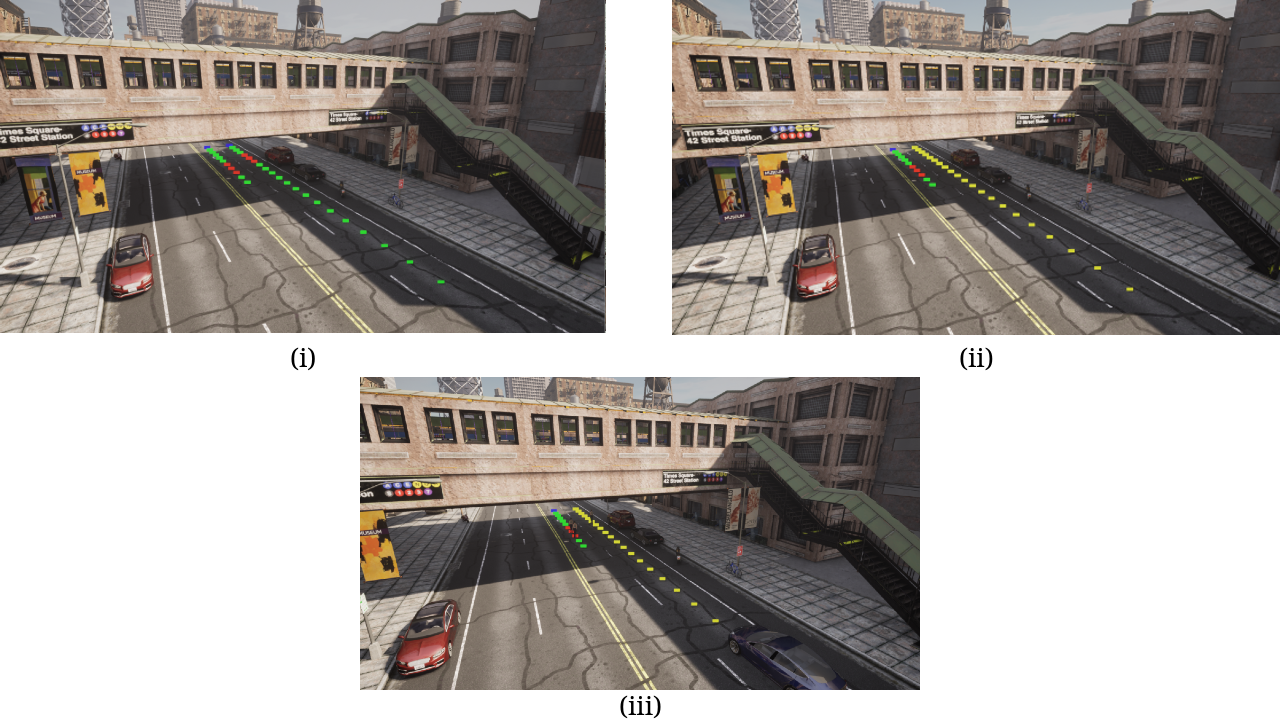
\includegraphics[width=\textwidth]{images/lane-change.png}
\begin{center} Figure 8: Carla scenario 17 \end{center}

It is inspired by \textit{17 - Obstacle avoidance without prior action} where the vehicle aims to avoid pedestrians whose presence is probabilistic by lane change.

 The right lane has an uncertain subgraph whose distribution is $0.2$, $0.5$, $0.2$. The left lane has an uncertain subgraph whose distribution is $0.7$, $0.8$, $0.8$. The vehicle decided to take the right lane. The results of 10 trials are as follows.

\begin{table}[h]
\centering
\begin{tabular}{cccc}
\toprule
\textbf{Trial} & \textbf{Left Penalty} & \textbf{Right Penalty} & \textbf{Positive} \\
\midrule
1 & 0.33 & 0.5 & \checkmark \\
2 & 0.5 & 0.5 & \ding{55} \\
3 & 0.25 & 0.5 & \checkmark \\
4 & 0.25 & 1.0 & \checkmark \\
5 & 0.25 & 1.0 & \checkmark \\
6 & 0.25 & 0.5 & \checkmark \\
7 & 0.33 & 0.33 & \ding{55} \\
8 & 0.25 & 1.0 & \checkmark \\
9 & 0.33 & 1.0 & \checkmark \\
10 & 0.33 & 0.5 & \checkmark \\
\bottomrule
\end{tabular}
\caption{Left and right lanes' penalties.}
\label{table:3}
\end{table}

As the vehicle is ahead of deciding between two lanes, both lanes decisions are emulated on Carla, where penalty is computed for both. If our mechanism led to a better penalty, i.e higher score, we declare the trial to be positively justifying our decision. In this case, it is reducing collisions with pedestrians. Here $80 \%$ of tested trials are positive.


\textbf{Break}

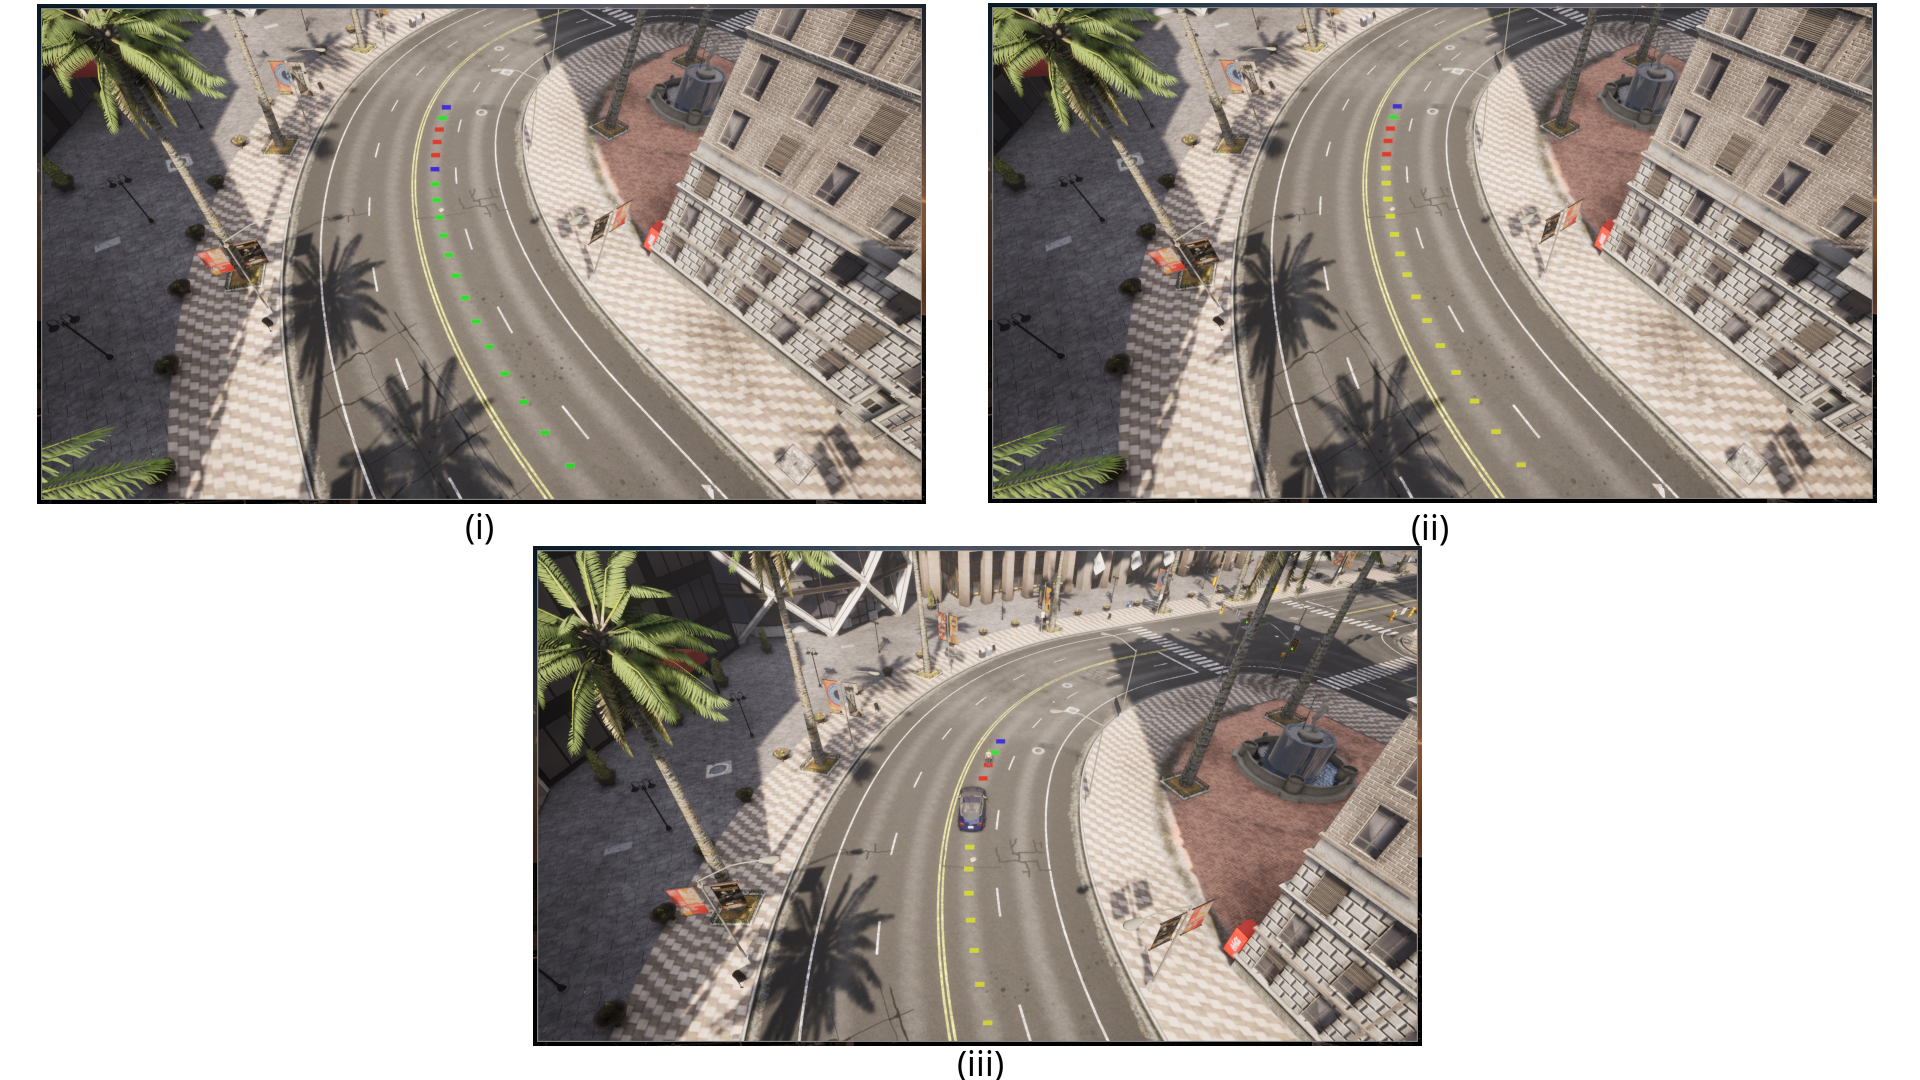
\includegraphics[width=\textwidth]{images/brake.png}
\begin{center} Figure 9: Carla scenario 16 \end{center}

It is inspired by \textit{16 - Longitudinal control after leading vehicle’s brake} where the vehicle brakes to avoid hitting pedestrians whose presence is probabilistic.

The uncertain subgraph distribution is $0.4, 0.1, 0.7$. The vehicle decided to brake before any uncertain vertex. The results of 10 trials are as follows.

\begin{table}[h]
\centering
\begin{tabular}{cccc}
\toprule
\textbf{Trial} & \textbf{Brake Penalty} & \textbf{Advance Penalty} & \textbf{Positive} \\
\midrule
1 & 0.5 & 0.5 & \ding{55} \\
2 & 1.0 & 0.5 & \checkmark \\
3 & 1.0 & 1.0 & \ding{55} \\
4 & 1.0 & 1.0 & \ding{55} \\
5 & 1.0 & 0.5 & \checkmark \\
6 & 0.5 & 0.5 & \ding{55} \\
7 & 0.5 & 0.33 & \checkmark \\
8 & 1.0 & 0.5 & \checkmark \\
9 & 1.0 & 0.5 & \checkmark \\
10 & 0.5 & 0.33 & \checkmark \\
\bottomrule
\end{tabular}
\caption{Brake versus advance penalties.}
\label{table:4}
\end{table}

As the vehicle is ahead of deciding between braking and advancing, both lanes decisions are emulated on Carla, where penalty is computed for both. We declare a trial to be positive similarly as we did before. In this case, it is reducing collisions with pedestrians. Here $60 \%$ of tested trials are positive.

It is notable to highlight the percentage here is decreased as the vehicle takes some time until it completely stops. Even if it decides to break at a way-point which is safe to be positioned in, acceleration effects may cause it to encroach into the uncertain zone. The odds of that increase if the vehicle is moving faster and an object turns out to be positioned near the boundaries of the uncertain zone.

We analyze how many meters are encroached from the uncertain graph, given distance between the vehicle and the uncertain graph, alongside vehicle's speed, during the moment of braking. In \textit{Image 3} the vehicle brakes only one waypoint, i.e 2 meters, from the uncertain graph colored in red.

\begin{center}
  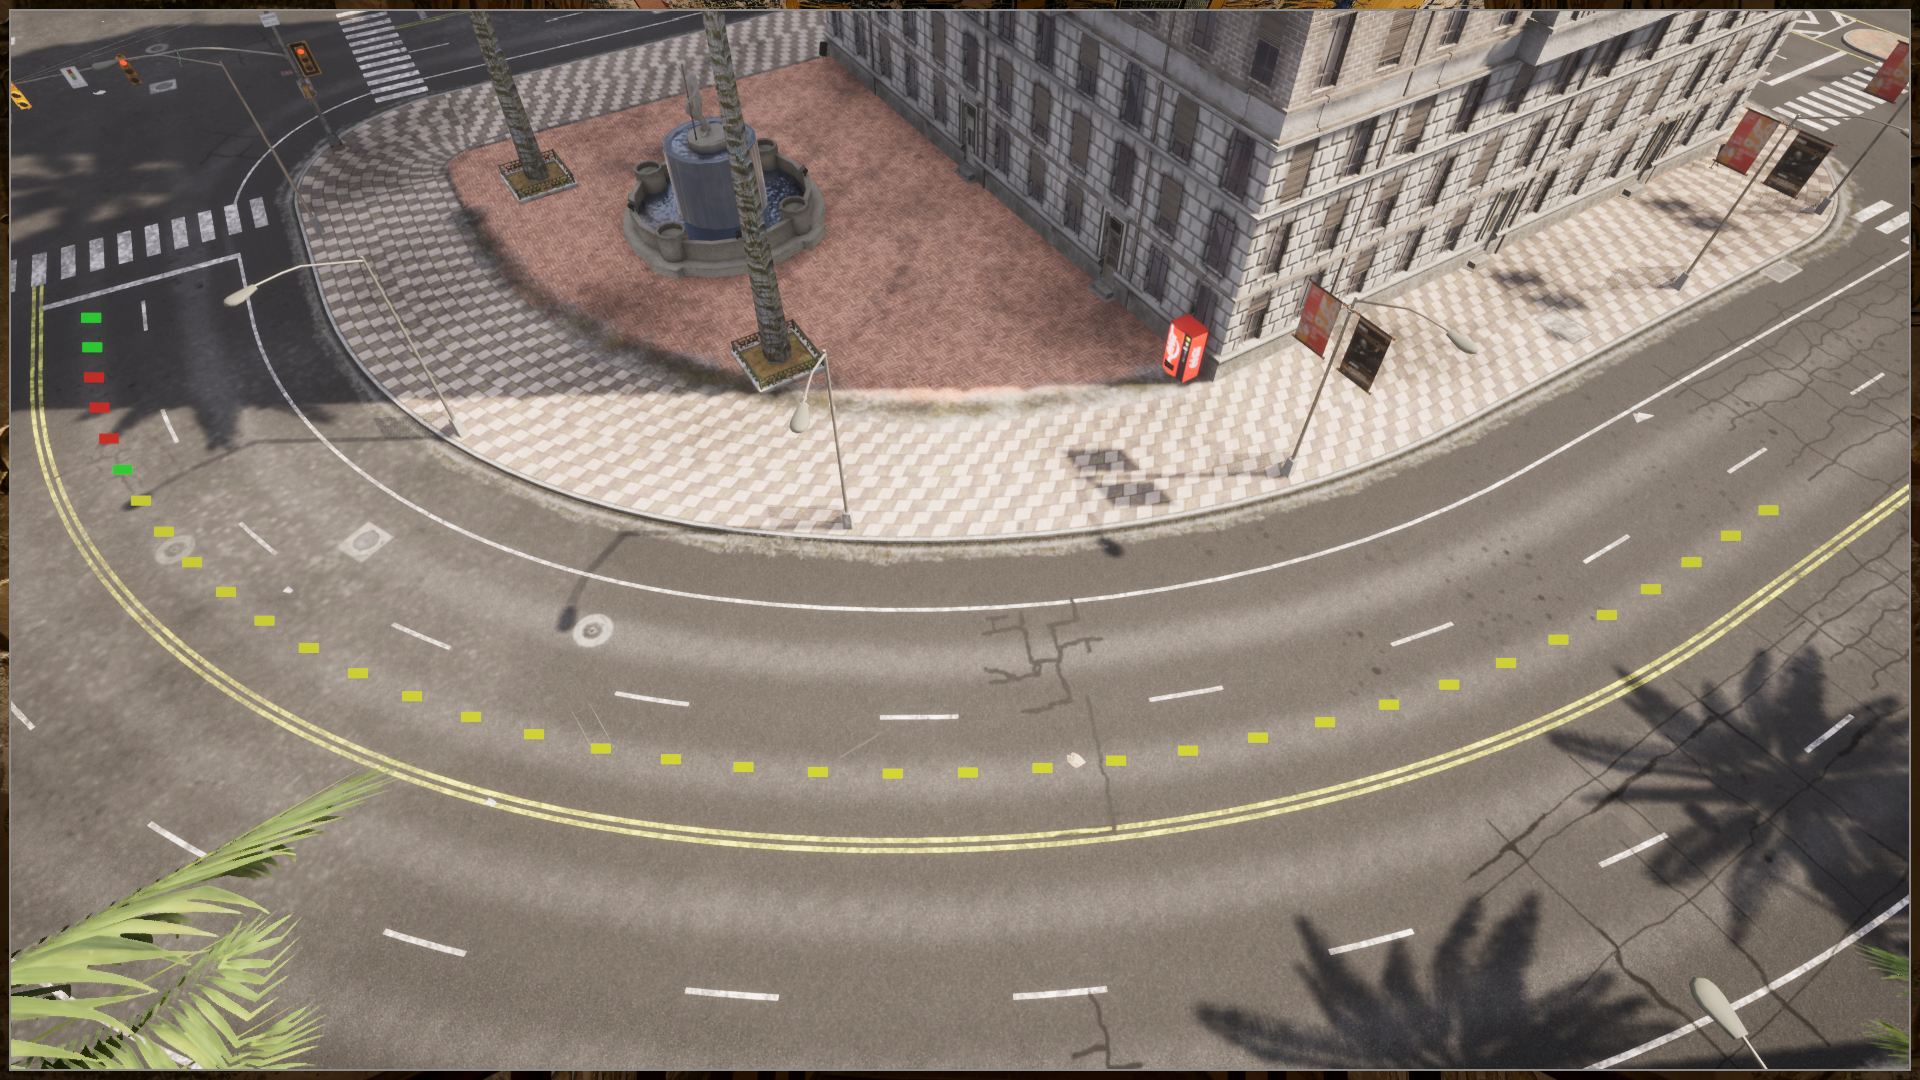
\includegraphics[width=0.5\textwidth]{images/brake-distance.png} \\
  Figure 10: Break analysis
\end{center}

The results of testing multiple values of distances and speeds are in \textit{Table 5}. For example, when the vehicle was 2 meters ahead of the uncertain graph with speed 60 km/h, it encroached 6 meters from the uncertain subgraph.

\begin{table}[h]
\centering
\begin{tabular}{cccc}
\toprule
\multicolumn{1}{c}{\textbf{Distance (m)}} & \multicolumn{3}{c}{\textbf{Speed (km/h)}} \\
\multicolumn{1}{c}{} & \textbf{30} & \textbf{45} & \textbf{60} \\
\midrule
2 & 2 & 4 & 6 \\
4 & 2 & 4 & 4 \\
8 & 0 & 0 & 0 \\
\bottomrule
\end{tabular}
\caption{Meters encroached given distances and speeds.}
\label{table:5}
\end{table}

Results suggest more than 4 meters are needed to avoid the uncertain subgraph upon braking.

In the \textit{Lane Change} scenario, modifying the distance and speed has no notable difference; the vehicle performs lane changes under these modified variables.

\textbf{Intersection}

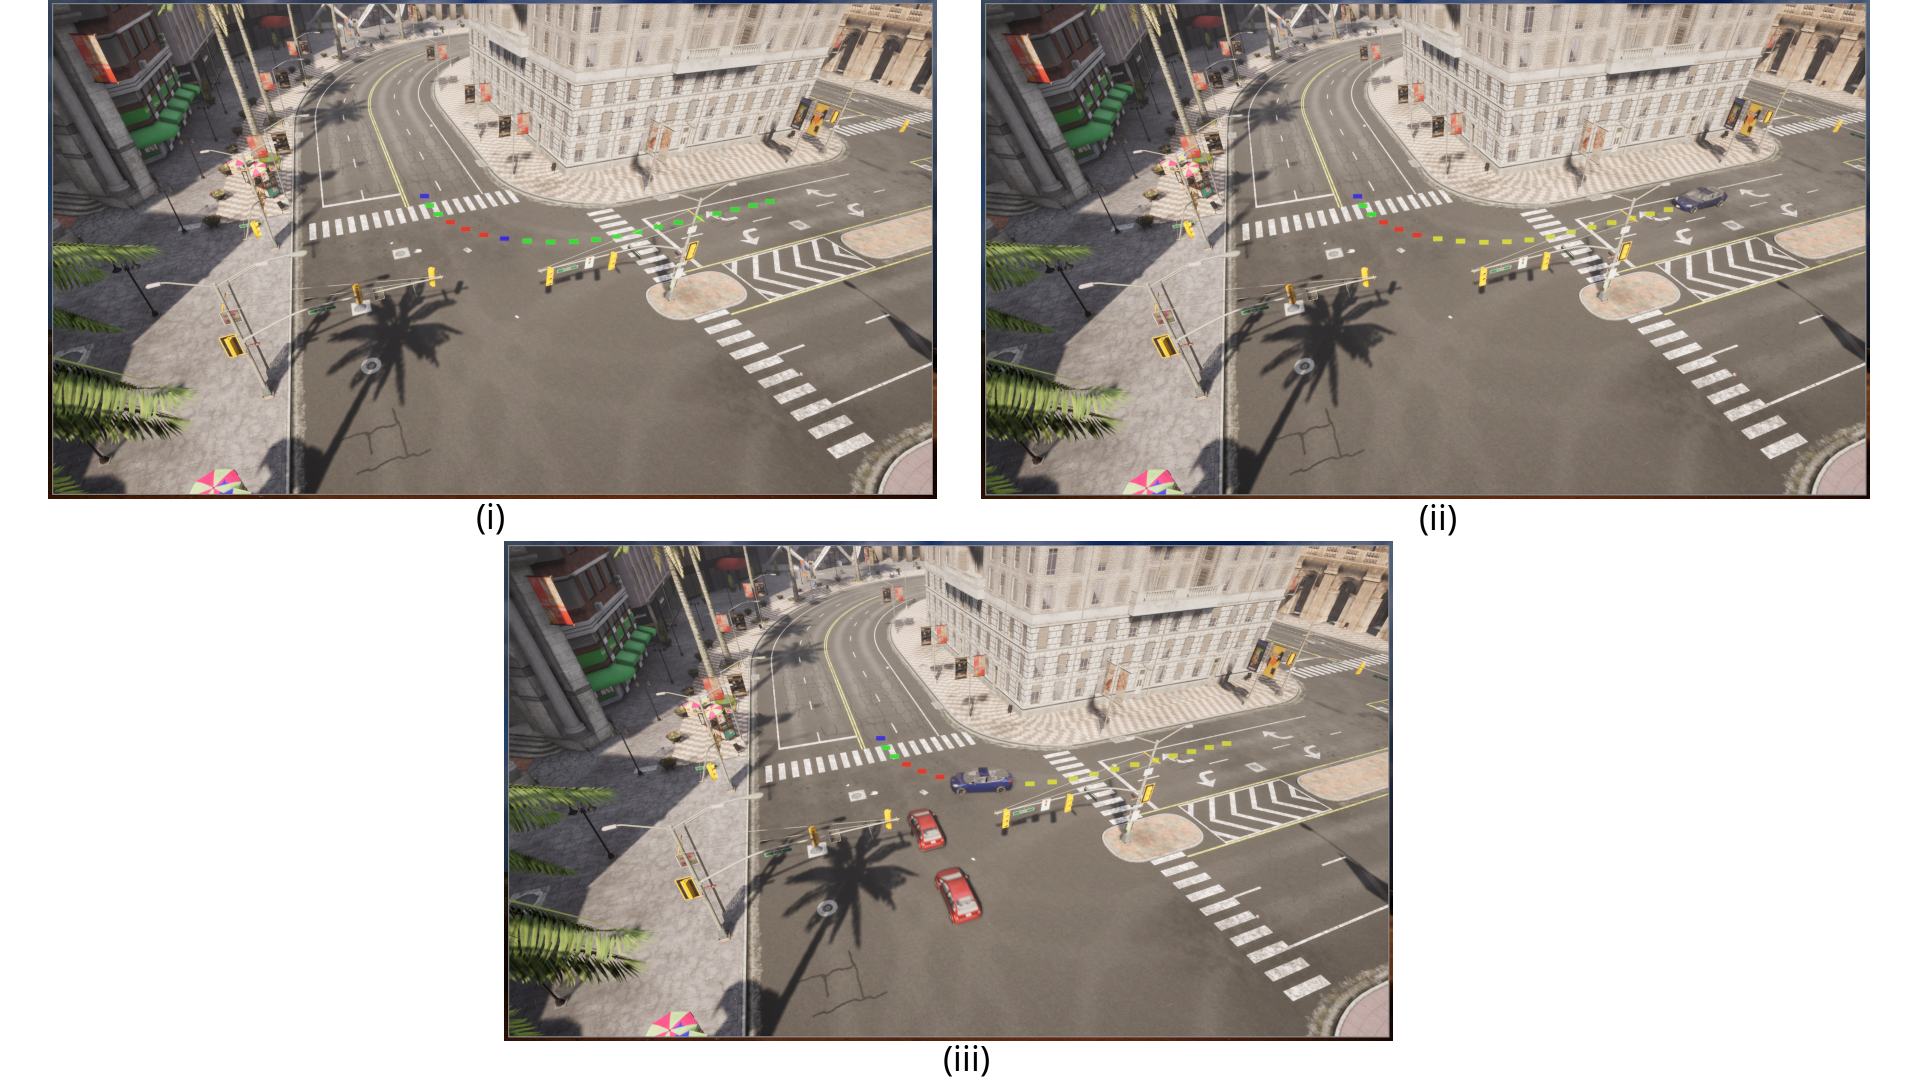
\includegraphics[width=\textwidth]{images/intersection.png}
\begin{center} Figure 11: Carla scenario 3 \end{center}

It is inspired by \textit{3 - Right turn at an intersection with crossing traffic.} where the vehicle breaks to avoid hitting crossing vehicles whose presence is probabilistic.

The uncertain subgraph distribution is $0.6, 0.5, 0.7$. The vehicle decided not to take the intersection. The results of 10 trials are as follows.

\begin{table}[h]
\centering
\begin{tabular}{cccc}
\toprule
\textbf{Trial} & \textbf{Intersection Penalty} & \textbf{Brake Penalty} & \textbf{Positive} \\
\midrule
1 & 0.59 & 1.0 & \checkmark \\
2 & 0.42 & 1.0 & \checkmark \\
3 & 0.59 & 1.0 & \checkmark \\
4 & 0.59 & 1.0 & \checkmark \\
5 & 0.59 & 1.0 & \checkmark \\
6 & 0.42 & 1.0 & \checkmark \\
7 & 1.0 & 1.0 & \ding{55} \\
8 & 1.0 & 1.0 & \ding{55} \\
9 & 0.42 & 1.0 & \checkmark \\
10 & 0.42 & 1.0 & \checkmark \\
\bottomrule
\end{tabular}
\caption{Brake versus intersecting penalties.}
\label{table:6}
\end{table}

As the vehicle is ahead of deciding between taking the intersection and braking, both decisions are emulated on Carla, where penalty is computed for both. We declare a trial to be positive similarly as we did before. In this case, it is reducing collisions with vehicles. Here $80 \%$ of tested trials are positive.

Observe the percentage here is increased, as the vehicle moves slowly at conjunctions, so it can break confidently.
